\documentclass[format=sigplan,authordraft]{acmart}
\usepackage{tikz-cd}
\usepackage{bbm}
\usepackage{ebproof}

% Macros {{{

\newcommand{\gcat}{\mathcal{G}_{\sqsubseteq}}
\newcommand{\kw}[1]{\ensuremath{ \mathsf{#1} }}
\newcommand{\ifr}[1]{\mathrel{[{#1}]}}
\newcommand{\bdot}{\boldsymbol{\cdot}}
\newcommand{\plays}[4]{{ {#1}_{{#2} \rightarrow {#3}}[{#4}] }}
\newcommand{\pplays}[3]{\plays{\bar{P}}{#1}{#2}{#3}}
\newcommand{\oplays}[3]{\plays{P}{#1}{#2}{#3}}
\newcommand{\htr}[3]{{ \{{#1}\} {#2} \{{#3}\} }}

%}}}

\title{Refinement-based game semantics} %{{{

\author{J\'er\'emie Koenig}
\affiliation{Yale University}
\email{jeremie.koenig@yale.edu}

\author{Zhong Shao}
\affiliation{Yale University}
\email{zhong.shao@yale.edu}

%}}}

\begin{document}

\maketitle

\section{Introduction} %{{{

\begin{color}{gray}
Contributions:
\begin{itemize}
\item A new understanding of nondeterminism in game semantics.
  Historically has been tricky and complicated.
  We believe this is due to conflating
  angelic nondeterminism
  (ranging over the possible choices of environment)
  which is always present in game models,
  vs. demonic nondeterminism
  (ranging over the possible choices of the system)
  which models of nondeterministic languages
  typically try to introduce.
\item Based on this,
  categories of games and strategies
  with refinement and a complete distributive lattice structure.
\item Can be used to provide a good semantics
  for the LTS of CompCertO.
  Show how to embed the stuff.
\item Use the algebraic flexibility of the result
  to recover techniques used in CertiKOS
  to formalize and work with
  certified abstraction layers.
\end{itemize}
\end{color}

Our approach draws upon a wide range of existing research.
In \S\ref{sec:bg},
we summarize the underlying concepts...

%}}}

\section{Background} %{{{

% Preamble {{{

The work presented in this paper
draws from a broad range of existing research.
This section summerizes the relevant aspects
of these various lines of work,
and outlines how we combine them
to develop
refinement-based game semantics.

%}}}

\subsection{Dual nondeterminism and refinement} \label{sec:refcal} %{{{

% Preamble {{{

Correctness properties for imperative programs
are often stated as triples of the form $\{P\} C \{Q\}$
asserting that
when the program $C$ is started in a state which
satisfies the predicate $P$ (the \emph{precondition}),
then the state in which $C$ terminates
will satisfy the predicate $Q$ (the \emph{postcondition}).
In the \emph{axiomatic} approach to programming language semantics,
inference rules
corresponding to the different constructions of the language
determine which triples are valid,
and the meaning of a program is identified with
the set of specifications $\{P\}\{Q\}$
which the program satisfies.

Axiomatic semantics
can accomodate nondeterminism in two different ways.
In the program $C_1 \sqcap C_2$,
a \emph{demon} will choose which of $C_1$ or $C_2$ is executed.
The demon will work against us,
so that if we want $C_1 \sqcap C_2$ to satisfy a given property,
we need to make sure we can deal with either choice.
This corresponds to the inference rule:
\[
  \begin{prooftree}
    \hypo{\htr{P}{C_1}{Q}}
    \hypo{\htr{P}{C_2}{Q}}
    \infer2{\htr{P}{C_1 \sqcap C_2}{Q}}
  \end{prooftree}
\]
Conversely,
in the program $C_1 \sqcup C_2$,
an \emph{angel} will decide whether $C_1$ or $C_2$ is executed.
If possible,
the angel will make a choice which validates
the correctness property.
This corresponds to the rules:
\[
  \begin{prooftree}
    \hypo{\{P\} C_1 \{Q\}}
    \infer1{\{P\} C_1 \sqcup C_2 \{Q\}}
  \end{prooftree}
  \qquad
  \begin{prooftree}
    \hypo{\{P\} C_2 \{Q\}}
    \infer1{\{P\} C_1 \sqcup C_2 \{Q\}}
  \end{prooftree}
\]
In other words,
a triple $\htr{P}{C}{Q}$
can be thought of as a \emph{game}
between the angel and the demon.
The angel resolves the $\sqcup$ choices,
whereas the demon resolves $\sqcap$.
The triple is valid if there is a winning strategy
for the angel.

%}}}

\paragraph{Distributivity} %{{{

Note that in this setup,
$\sqcap$ and $\sqcup$ distribute over each other.
More precisely, for all $P, C_1, C_2, C_3, Q$:
\begin{align*}
  \htr{P}{C_1 \sqcap (C_2 \sqcup C_3)}{Q} &\Leftrightarrow
    \htr{P}{(C_1 \sqcap C_2) \sqcup (C_1 \sqcap C_3)}{Q} \\
  \htr{P}{C_1 \sqcup (C_2 \sqcap C_3)}{Q} &\Leftrightarrow
    \htr{P}{(C_1 \sqcup C_2) \sqcap (C_1 \sqcup C_3)}{Q}
\end{align*}
Consider the first equivalence above.
If the angel has a winning strategy for
the left-hand side triple,
they can win both $\htr{P}{C_1}{Q}$
and either $\htr{P}{C_2}{Q}$ or $\htr{P}{C_3}{Q}$.
Although the right-hand side triple
reverses the angel and demon's choices,
the angel can preemptively choose the left or right
disjunct depending on whether they can win
$\htr{P}{C_2}{Q}$ or $\htr{P}{C_3}{Q}$.
Likewise, if the angel can win the right-hand side,
then they have a winning strategy for the left-hand as well.
The second equation corresponds to a similar situation
where the angel and demon have been exchanged.

%}}}

\paragraph{Program refinement} %{{{

Instead of proving program correctness in one go,
\emph{stepwise refinement} techniques use a more incremental approach
centered on the notion of program refinement.
A refinement $C_1 \sqsubseteq C_2$
means that any specification satisfied by $C_1$
will also be satisfied by $C_2$:
\[
    C_1 \sqsubseteq C_2 \: := \:
    \forall P Q \cdot
      \{P\} C_1 \{Q\} \Rightarrow
      \{P\} C_2 \{Q\}
\]
We say that $C_2$ refines $C_1$
or that $C_1$ is refined by $C_2$.

Typically,
under such approaches,
the language will be extended with constructions
allowing the user to describe
abstract, declarative specifications as well as
concrete, executable programs.
The goal will then be to establish
a sequence of refinements
$C_1 \sqsubseteq \cdots \sqsubseteq C_n$
to show that a program $C_n$ involving
only executable constructions
correctly implements a specification $C_1$
which may be stated in much more abstract terms.

Angelic and demonic choice
are particularly interesting in this light,
because they respectively give the
least upper bound and greatest lower bound
with respect to $\sqsubseteq$.
As a specification, $C_1 \sqcup C_2$
requires an implementation to refine
\emph{both} $C_1$ and $C_2$:
\[
    C_1 \sqcup C_2 \sqsubseteq C \: \Leftrightarrow \:
    C_1 \sqsubseteq C \: \wedge \: C_2 \sqsubseteq C \,,
\]
and $C_1 \sqcap C_2$
allows an implementation to refine
either:
\[
    C_1 \sqcap C_2 \sqsubseteq C \: \Leftarrow \:
    C_1 \sqsubseteq C \: \vee \: C_2 \sqsubseteq C \,.
\]

Note that in the context of \emph{specifications}
(on the left of $\sqsubseteq$),
the terminology of \emph{angelic} and \emph{demonic}
choices are somewhat counterintuitive
because they work in the opposite way:
demonic choices in the specification gives us more
implementation freedom,
and help us establish refinement,
whereas angelic choices make the specification
stronger and more difficult to implement.
Intuitively,
the \emph{user} of a specification
will need to be ready to handle any demonic choice
made in that specification.
The component's implementer
will have more freedom because they \emph{are} the demon.
Conversely,
angelic choice requires the implementer to be
ready to behave appropriately
no matter which alternative the user decides to rely on.
In that sense,
we will often think of demonic choices as
choices of the \emph{system} we are considering,
and think of angelic choices as
choices of its \emph{environment}.

%}}}

\begin{color}{gray}
\paragraph{Unbounded choice} %{{{

Angelic and demonic choice
generalize to infinitary constructions,
which subsume many familiar ones.
For instance:
\begin{align*}
  \kw{abort} &:= \bigsqcup \varnothing &
  \{ P \} &:= \bigsqcup \{ \kw{skip} \mid P \} \\
  \kw{magic} &:= \bigsqcap \varnothing &
  [ P ] &:= \bigsqcap \{ \kw{skip} \mid P \}
\end{align*}
The program $\kw{abort}$ represents unconditional failure;
it is the least element with respect to $\sqsubseteq$
and can also be seen to denote completely unspecified behavior.
Conversely, $\kw{magic}$ refines \emph{any} specification,
and can be seen as the unimplementable behavior.
The \emph{assertion} $\{P\}$ checks whether
the predicate $P$ holds in the current state,
and behaves as either $\kw{skip}$ or $\kw{abort}$
depending on the result.
Dually, the \emph{assumption} $[P]$ behaves as
$\kw{skip}$ or $\kw{magic}$ depending on whether $P$ holds.

We will treat divergence as a catastrophic failure
and conflate it with \kw{abort}.
Under this approach,
we can define iteration as follows:
\[
  \kw{while} \: P \: \kw{do} \: C \: \kw{od} \: := \:
    \bigsqcup_{n \in \mathbb{N}}
    (\{\neg P\}; C)^n ; \{P\}
\]
where $C^n$ is the $n$-fold sequential composition
$C ; C ; \cdots ; C$.

%In the presence of dual nondeterminism,
%generalized programs and specifications are sometimes
%known collectively as \emph{contracts}.
%The combination of angelic and demonic choices

%}}}
\end{color}

\paragraph{The refinement calculus} %{{{

These basic ingredients have been studied systematically
in the \emph{refinement calculus},
dating back to Ralph-Johan Back's 1978 PhD thesis \cite{backthesis}.
In its modern incarnation \cite{refcal},
the refinement calculus
subsumes programs and specifications with \emph{contracts}
featuring unbounded angelic and demonic choices.
These choice operators
constitute a completely distributive lattice
with respect to the refinement order.

Dijkstra's \emph{predicate transformer} semantics
are a natural fit for the refinement calculus,
but other approaches are possible.
For instance,
the understanding of contracts as a game between
the angel and the demon
can be formalized to provide a form of
game semantics for the refinement calculus.

[Mention the refinement calculus \emph{hierarchy},
where simpler models (state transformers, relations)
can be embedded in more general ones
(predicate transformers)
in a structure-preserving way,
allowing to reason about simpler components
in a simpler, stronger framework,
but connecting them in a more general one.
This is exactly what we want for
large-scale verification
and connecting things verified through different approaches
together.]

Like all methods in the lineage of Hoare logic
it only applies to imperative programs,
with no side-effects beyond changes to the global state.
Recent research has attempted to extend the paradigm
to a broader setting,
and the present work can be understood
as a step in this direction as well.

%}}}

\paragraph{Dually nondeterministic functions} %{{{

Morris and Tyrrell were able to extend
the lattice-theoretic approach used in the refinement calculus
to functional programming
\cite{augtyp,dndf,cspdnd}:
if types are interpreted as posets,
dual nondeterminism can be added at the type level
using the \emph{free completely distributive} completion.
This allows dual nondeterminism to be used
in a variety of new contexts.

A completely distributive lattice $L$ is a
free completely distributive completion of
a poset $C$ is there is
a monotonic function $\phi : C \rightarrow L$
such that
for any completely distributive lattice $M$
and monotonic function $f : C \rightarrow M$,
there exists a unique complete morphism $f^*_\phi : L \rightarrow M$
such that $f^*_\phi \circ \phi = f$:
\[
  \begin{tikzcd}
    C \arrow[r, "\phi"] \arrow[rd, "f"'] &
    L \arrow[d, "f^*_\phi", dashed] \\ & M
  \end{tikzcd}
\]
A free completely distributive lattice over a poset
always exists and it is unique up to isomorphism.
We write $\mathbf{FCD}(C)$ for
the free completely distributive lattice over $C$.

In \cite{augtyp}, Morris shows that
the free completely distributive lattice over $(A, \le)$
can be constructed as one of:
\begin{align*}
  \mathbf{FCD}(A, {\le}) &:= \mathcal{D} \mathcal{U}(A, {\le}) &
  \mathbf{FCD}(A, {\le}) &:= \mathcal{U} \mathcal{D}(A, {\le}) \\
  \phi(a) &:= {\downarrow}{\uparrow} a &
  \phi(a) &:= {\uparrow}{\downarrow} a \,.
\end{align*}
In the expressions above,
$\mathcal{D}$ and $\mathcal{U}$
are themselves completions.
A \emph{downset} of a poset $(A, {\le})$
is a subset $x \subseteq A$ satisfying:
\[
  \forall \, a, b \in x \,.\,
          a \le b \wedge b \in x \Rightarrow a \in x \,.
\]
Unions and intersections preserve this property,
giving rise to the \emph{downset lattice} $\mathcal{D}(A, {\le})$,
which consists of all downsets of $(A, {\le})$,
ordered by set inclusion (${\subseteq}$) with
unions as joins and intersections as meets.
The dual \emph{upset lattice} $\mathcal{U}(A, {\le})$
is ordered by set containement (${\supseteq}$) with
intersections as joins and unions as meets.

Categorically speaking,
$\mathbf{FCD} : \mathbf{Poset} \rightarrow \mathbf{CDL}$
is the left adjoint to the forgeful functor
$U : \mathbf{CDL} \rightarrow \mathbf{Poset}$
from the category $\mathbf{CDL}$
of completely distributive lattices and complete homomorphisms
to the category $\mathbf{Poset}$
of partially ordered sets and monotonic functions.
As such, $U \! \circ \mathbf{FCD}$ is a monad over $\mathbf{Poset}$,
and can be used to model dual nondeterminism
as an effect.

In order to specify effectful computations,
we will extend this monad by adding
arbitrary, uninterpreted effects.

%}}}

%}}}

\subsection{Effect signatures} %{{{

The framework of \emph{algebraic effects}
models computations as terms in an algebra
whose operations represent effects:
a term $e(x_1, \ldots x_n)$
represents a computation which first
triggers an effect $e$,
then goes on as a computation derived from
the subcomputations $x_1, \ldots x_n$.
For example,
the term:
\[
    \kw{readbit}(
      \kw{print}["\text{Hello}"](\kw{done}),
      \kw{print}["\text{World}"](\kw{done}))
\]
could denote a computation which
first reads one bit of information,
then depending on the result
causes the words ``Hello'' or ``World'' to be output,
and terminates.

Under this approach,
effects can be described as generalized algebraic theories:
a signature gives the set of operations and their arities,
and a set of equations describes their behaviors
by specifying which computations are equivalent.
For example above uses a signature with the operations
$\kw{done}$ of arity $0$,
$\kw{readbit}$ of artiry $2$,
and a family of operations $(\kw{print}[s])_{s \in \kw{string}}$
of arity $1$.
An equation for this signature is:
\[
    \kw{print}[s](\kw{print}[t](x)) =
    \kw{print}[st](x) \,,
\]
which indicates that
printing the string $s$ followed by
printing the string $t$ is equivalent to
printing the string $st$ in one go.

In this work,
we use effect signatures to represent
the possible external interactions
of a computation,
but we will not use equational theories.
The \emph{interaction monad} $\mathcal{I}_E$
presented in \S\ref{sec:intmonad}
combines the dual nondeterminism of $\mathbf{FCD}$ with
uninterpreted effects taken from
an arbitrary effect signature $E$.
\begin{color}{gray}
We will however make it possible to interpret effects through
\emph{effect handlers}.
\end{color}

%}}}

\subsection{Game semantics} \label{sec:strat} %{{{

Game semantics is an approach to denotational semantics
which interprets types as two-player games
between a program component (the \emph{system})
and the context in which it appears (the \emph{environment}).
Terms of a given type are then interpreted as
strategies for the corresponding game,
specifying for each position in the game
the next action to be taken by the system.

An early success of this approach,
building on game models developped for
fragments of linear logic,
was the formulation of the first satisfactory
full abstraction results
for the functional programming language PCF.
Since then,
game semantics has been extended to
model a wide variety of language features.

\paragraph{Traditional strategy models} %{{{

The \emph{plays} of a game are sequences of moves;
they both identify a position in the game
and describe the succession of actions that led to it.
Most game models of sequential computation
use \emph{alternating} games,
where in any play
the system and environment each contribute
every other move.
It is also common to require the environment to play first
and to focus on plays of even length,
which specify which action the system took
in response to the latest environment move.
We will write $P_G$ for the set of plays of the game $G$,
partially ordered by the prefix relation $\sqsubseteq$.

Traditionally \cite{gamesem99},
strategies are defined as
prefix-closed sets of plays,
so that strategies $\sigma \in \mathcal{S}_G$
for the game $G$ are downsets of $P_G$
satisfying certain requirements:
\[
    \mathcal{S}_G \subseteq
    \mathcal{D}(P_G, {\sqsubseteq})
\]
A common constraint is that $\sigma \in \mathcal{S}_G$
should not contain two plays $s m_1, s m_2 \in \sigma$
where $m_1$ and $m_2$ are distinct moves of the system.
This is usually understood as
enforcing \emph{system} determinism:
given a set of environment choices,
there is only one possible behavior for the system.
Therefore,
relaxing this constraint has usually been understood
as the first step toward modeling nondeterministic systems
\cite{gsfnd}.
However,
looking at the situation through the lens of
the refinement calculus and dual nondeterminism,
we will come to a different conclusion,
understanding this requirement as
\emph{environment determinacy}.

As a poset completion,
the downset lattice
$\mathcal{D}(P_G, {\sqsubseteq})$
can be understood as
the \emph{free completely distributive join-semilattice}.
A play $s \in P_G$ can be lifted to a strategy
${\downarrow} s \in \mathcal{D}(P_G, {\sqsubseteq})$:
\[
    {\downarrow} s := \{ t \in P_G \mid t \sqsubseteq s \}
\]
Set inclusion corresponds to refinement of strategies,
and following the approach outlined in \S\ref{sec:refcal},
the lattice structure provides
arbitrary angelic and demonic choice operators.

Anglic nondeterminism
allows us to range over all possible choices of the environment
and record the resulting plays.
For instance,
a very simple strategy which computes
the double of a natural number $n$
provided by the environment
can be written as:
\[
  \sigma :=
    \bigcup_{n \in \mathbb{N}} {\downarrow}(n \cdot \underline{2n}) =
    \{ \epsilon, \: n, \: n \cdot \underline{2n} \mid n \in \mathbb{N} \}
\]
If we want $\sigma$ to be a looser specification,
so that an acceptable implementation
would be allowed to provide any answer in the interval
$[2n - 1, 2n + 1]$,
this strategy model becomes insufficient
because the downset lattice does not add enough meets,
forcing the specification to become
much coarser:
\[
  \sigma :=
    \bigcup_{n \in \mathbb{N}} \:
    \bigcap_{-1 \le \delta \le 1}
    {\downarrow}(n \cdot \underline{2n+\delta}) =
    \{ \epsilon, n \mid n \in \mathbb{N} \} \,,
\]
We will remedy this by using a richer completion.

%}}}

\paragraph{Dually nondeterministic strategies} %{{{

Our approach to nondeterminism in game semantics
will be to substitute $\mathbf{FCD}$ for $\mathcal{D}$
in the construction of strategies presented in \S\ref{sec:strat}.
In this framework,
the more permissive strategy
can be written as:
\[
  \sigma :=
    \bigsqcup_{n \in \mathbb{N}}
    \bigsqcap_{-1 \le \delta \le 1}
    \phi(n \cdot \underline{2n + \delta})
\]
Because of the properties of $\mathbf{FCD}$,
the strategy $\sigma$ will retain
not only angelic choices,
but demonic choices as well,
corresponding to the possible behaviors
of the system.
%In particular, we have that:
%\[
%    \sigma \nsqsubseteq \bigsqcup_{n \in \mathbb{N}} n
%\]

\begin{color}{gray}

The precise construction we use for $\mathbf{FCD}$ is irrelevant,
and in general it will be much more intuitive
to think of it by its defining property as a free object and
write its elements in terms of $\phi$, $\sqcap$, $\sqcup$, and $-_\phi^*$
rather than use any concrete representation.
However, to work out this example
we will use the second construction of $\mathbf{FCD}$ above,
where $\mathcal{D}(A, {\le})$ appears,
making the connection with traditional strategy models
more easily apparent.
In this case, we obtain:
\[
    \sigma =
    \{ \chi \in \mathcal{D}(P_G, {\sqsubseteq}) \mid
       \exists \vec{\delta} \,
       \forall n \,.\,
       (n \cdot \underline{2n + \delta_n}) \in \chi \}
\]
In this representation,
each $\chi \in \sigma$
is a prefix-closed set of plays,
emulating the traditional strategies described in \S\ref{sec:strat}
and corresponding to a situation where all of the system's choices
have been fixed (here as $\vec{\delta} \in [-1,1]^\mathbb{N}$).

\end{color}

%}}}

\paragraph{Determinacy} %{{{

How should we understand
the traditional strategy containing $\{ sm_1, sm_2 \}$
when $m_1$ and $m_2$ are system moves?
Under our interpretation,
this does not correspond to
system nondeterminism;
\emph{by construction},
such nondeterminism cannot occur,
and indeed
${\downarrow} s m_1 \sqcap {\downarrow} s m_2 =
 {\downarrow} s \notni
 s m_1, s m_2$.
Instead,
we interpret this as an \emph{unobservable}
environment choice
between the outcomes $s m_1$ and $s m_2$.

Can happen as consequence of abstraction.
Perhaps an assembly spec says
the outcome of a function should depend on the value of some
register which is considered irrelevant by the C calling convention.
If we try to lift this spec to the C level
we will get $s m_1 \sqcup s m_2$.
This can never be implemented by a C program
since C language semantics are determinate in the environment
(and deterministic for the system).

[One question is whether
some form of determinate strategies
can still form a lattice
(with say, $sm_1 \sqcup sm_2 = s \top$).]

%}}}

%}}}

%}}}

\section{Interaction monad} \label{sec:intmonad} %{{{

In the following,
we present a game semantics equipped with a notion of refinement,
and which features both angelic and demonic nondeterminism.
This framework is based on an \emph{interaction monad} $\mathcal{I}_E$
modelling computations which can interact with their environment
according to the elementary game $E$.
We use this monad to build our strategy model for the
arrow games $E \rightarrow F$,
and show how to interpret the operational semantics
and simulation conventions defined in \S\ref{sec:compcert}.
We conclude by defining a notion of \emph{semantic linking}
similar to the one used in Compositional CompCert.

\subsection{Effect signatures} %{{{

In this work we focus on the the first aspect
of the framework;
signatures can be specified as follows.

\begin{definition}
An \emph{effect signature}
is a set $E$ of operations
together with a mapping $\kw{ar}$,
which assigns to each $e \in E$ a set $\kw{ar}(e)$
called the \emph{arity} of $e$.
We will use the notation
$E = \{ e_1 : \kw{ar}(e_1), e_2 : \kw{ar}(e_2), \ldots \}$
to describe effect signatures.
\end{definition}

Terms are constructed by
applying function symbols $e \in E$
to subcomputations given for each $r \in \kw{ar}(e)$.
In simple cases,
the computation $e(x_r)_{r \in \kw{ar}(e)}$
first triggers an effect $e$;
the context then chooses $k$
and resumes the computation as $x_r$.
For example,
the following effect signature
models a very basic input/output facility:
\[
  E_\kw{io} :=
    \{ \kw{readbit} : \mathbbm{2}, \:
       \kw{writebit}[n] : \mathbbm{1} \mid
       n \in \mathbbm{2} \}
\]
A computation which writes a zero,
reads one bit, echoes its complement
and continues as the computation $k$
can be written as:
\[
  \kw{writebit}[0](
    \kw{readbit}(
      \kw{writebit}[1](k),
      \kw{writebit}[0](k)))
\]
\[
  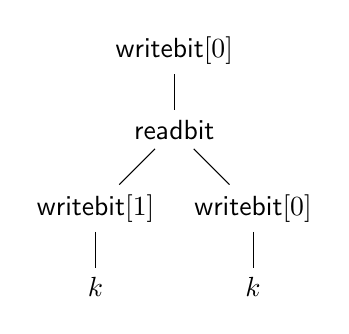
\begin{tikzpicture}
    \node (W) at (0,0) {$\kw{writebit}[0]$};
    \node (R) at (0,-1) {$\kw{readbit}$};
    \node (W0) at (-1,-2) {$\kw{writebit}[1]$};
    \node (W1) at (+1,-2) {$\kw{writebit}[0]$};
    \node (K0) at (-1,-3) {$k$};
    \node (K1) at (+1,-3) {$k$};
    \path (W) edge (R);
    \path (R) edge (W0);
    \path (R) edge (W1);
    \path (W0) edge (K0);
    \path (W1) edge (K1);
  \end{tikzpicture}
\]
Note the similarity with strategy trees.

\begin{definition}
We define the effect signature
$\mathbf{1} := \varnothing$.
For a family of effect signatures $(E_i)_{i \in I}$,
we define:
\[
  \bigotimes_i E_i := \{ (i, e) : \kw{ar}(e) \mid i \in I, e \in E_i \}
\]
\end{definition}

For example,
the signature above can be decomposed as:
\[
    E_\kw{io} = \{ \kw{readbit} : \mathbbm{2} \} \otimes
      \{ \kw{writebit}[n] : \mathbbm{1} \mid n \in \mathbbm{2} \}
\]

[Note somewhere:]
This coincides with the cartesian product in $\gcat^i$
(where there is only one top-level question
so a strategy for $A \multimap \bigotimes_i B_i$
is completely defined
by specifying its behavior for each of the $B_i$),
but it is only a monoidal tensor in $\gcat$
(where subsequent questions in the different $B_i$'s
may interact with each other).

We will interpret an effect signature $E$
as a very simple game,
consisting of
one question $m \in E$ from the environment followed by
one answer $n \in \kw{ar}(e)$ from the system.
In traditional terms,
this corresponds to the arena specified by:
\[
    \star \vdash m \vdash n \qquad
      (m \in E, \: n \in \kw{ar}(m))
\]
The connection with
effect algebras will become clear in \S\ref{sec:intmonad}.

%}}}

\subsection{Definition} \label{sec:monad:def} %{{{

First,
we define the monad $\mathcal{I}_E(A)$
at the heart of our game semantics.
To this end,
we first define the sets of plays $P_A(V)$
for the elementary game $A$ with return values in $V$.
Plays already constitute a monad,
however we emulate the approach taken in \cite{cspdnd}
and take their \emph{completely distributive lattice completion}
to obtain a strategy domain featuring dual nondeterminism.

When $\kw{P}$ is to play,
it can either terminate with a return value $v \in A$,
or make a move $m \in M_E^\kw{P}$ and pass control to $\kw{O}$,
which is then free to resume the computation with
a move $n \in M_E^\kw{O}$ of its own,
or to abandon the computation.
Accordingly,
the plays $s \in P_E(A)$
for an elementary game $E$ and a return type $A$
are defined inductively as:
\[
  s \in P_E(A) ::= v \mid \underline{m} \mid \underline{m} ns \,,
\]
where $v \in A$, $m \in M_E^\kw{P}$ and $n \in M_E^\kw{O}$.
The prefix ordering
${\sqsubseteq} \subseteq P_E(A) \times P_E(A)$
is a natural refinement relation on plays,
and can be defined
as the smallest relation satisfying:
\[
  v \sqsubseteq v \,, \qquad
  \underline{m} \sqsubseteq \underline{m} \,, \qquad
  \underline{m} \sqsubseteq \underline{m}t \,, \qquad
  \begin{prooftree}
    \hypo{s \sqsubseteq t}
    \infer1{\underline{m}s \sqsubseteq \underline{m}t}
  \end{prooftree} \,.
\]

With refinement in mind,
the traditional construction of strategies
as prefix-closed sets of plays
can be understood as a lattice completion of the poset
$\langle P_E(A), {\sqsubseteq} \rangle$,
augmenting plays with angelic nondeterminism:
the behavior of a component is characterized completely
by having an angel range over all possible behaviors of the environment
and collecting the resulting plays in a set.
Prefix closure is a natural restriction because,
if $s \sqsubseteq t$ and the play $t$ is a possible outcome,
then the environment may also have stopped earlier,
resulting in the outcome $s$ instead.
Writing:
\[
  \mathcal{D}(A, {\le}) :=
    \langle
    \{ S \in \mathcal{P}(A) \mid
        \forall x, y \in A \,.\,
           x \le y \wedge y \in S \Rightarrow x \in S \},
    {\subseteq}
    \rangle
\]
for the set of down-closed subsets of $\langle A, {\le} \rangle$
ordered by inclusion,
this traditional construction can be given as
$\mathcal{S}_E(A) :=
\langle \mathcal{D}(P_E(A), {\sqsubseteq}), {\subseteq} \rangle$.

Note that this point of view suggests a new interpretation
of the determinism requirement usually placed on strategies
mentioned in \S\ref{sec:mainideas:gs:strat}.
Consider
two plays $s\underline{m_1}$ and $s\underline{m_2}$
differing only in the recorded behavior of the system
($m_1 \neq m_2$).
It is tempting to assume that
a strategy containing both of them
denotes the behavior of a non-deterministic system.
However,
under our interpretation,
while the difference between $s\underline{m_1}$ and $s\underline{m_2}$
manifests itself as the obervation of different system behaviors,
these differences are still the result of \emph{angelic} choices,
in other words they are the result of hidden choices made by the
environment.

In the model we have considered so far,
the system itself is always deterministic.
By excluding plays which differ only in their system component,
we have not enforced the determinism of the system,
but rather the \emph{determinacy} of the environment,
in the sense that angelic choices should always be observable
as distinct \kw{O}-moves.
Consequently,
an appropriate model of nondeterministic systems
cannot be obtained simply by relaxing this requirement,
and indeed in \cite{gsfnd} this approach
prevents the modelling of unbounded nondeterminism.

Instead,
we adapt the approach used in \cite{augtyp}
and use the \emph{free completely distributive lattice}
over $\langle P_E(A), {\sqsubseteq} \rangle$
to endow strategies with both angelic and demonic nondeterminism.
Writing:
\[
  \mathcal{U}(A, {\le}) :=
    \langle
    \{ S \in \mathcal{P}(A) \mid
        \forall x, y \in A \,.\,
           x \le y \wedge x \in S \Rightarrow y \in S \},
    {\supseteq}
    \rangle
\]
for the set of up-closed subsets of $\langle A, {\le} \rangle$
ordered by containement,
the free completely distributive lattice over a poset
can be defined as the composition
$\mathcal{U}(\mathcal{D}(A, {\le}), {\subseteq})$.
We define our interaction monad as follows.

\begin{definition}
The \emph{interaction monad}
for an elementary game $E$
maps the type $A$ to the type of \emph{interactive behaviors}
$\mathcal{I}_E(A)$ where:
\[
  \langle \mathcal{I}_E(A), {\sqsubseteq} \rangle :=
    \mathcal{U}(\mathcal{S}_E(A)) \,.
\]
\end{definition}

In this construction,
the \emph{inner} sets $S \in \mathcal{S}_E(A)$
are similar to traditional strategies and
can be interpreted in the usual way,
noting however that their consistuent plays
are the result of angelic choices
no matter how and when these choices become observable.
The \emph{outer} set records \emph{demonic} choices,
and can be interpreted as follows:
the presence in the outer set $x \in \mathcal{I}_E(A)$
of an inner set $S \in x$
indicates that the demon has a strategy
to ensure that the outcome remains in $S$
no matter what the angel does.
It is natural for $x$ to be up-closed:
if $S \subseteq T$ and the demon can make sure
the outcome is contained in $S$,
then the outcome will be contained in $T$ as well.

\subsection{Operations}

\subsubsection{Termination}

The unit $\eta^E_A : A \rightarrow \mathcal{I}_E(A)$
of the interaction monad
assigns to a value $v \in A$ the computation
which simply returns $v$ immediately.
Because the environment is never in control,
the system can ensure that the outcome is always
the terminated play $v$.
In other words,
the demon has a strategy to ensure that the outcome is in $S$
whenever $v \in S$:
\[
  \eta^E_A(v) :=
    \{ S \in \mathcal{D}(P_E(A), {\sqsubseteq}) \mid v \in S \} \,.
\]

\subsubsection{Nondeterminism}

The refinement lattice over $\mathcal{I}_E(A)$
provides unbounded demonic choices
in the form of arbitrary meets
(realized as the union of the outer sets),
and unbounded angelic choices
in the form of arbitrary joins
(realized as the intersection of the outer sets).
A refinement $x \sqsubseteq y$ expresses that
$y$ offers fewer demonic choices and more angelic choices than $x$.

In particular,
the least element $\bot = \bigsqcup \varnothing$
corresponds to a situation where the environment has no choices
and the computation cannot be resumed.
It can be refined by any other computation and
we will use it to interpret undefined behaviors and silent divergence.
Conversely,
the greatest element $\top = \bigsqcap \varnothing$
corresponds to the \emph{magic} behavior
which refines all others:
the system has no choices,
therefore any behavior is vacuously satisfactory.

Another special case of angelic choice is
the \emph{assertion} of a proposition $P$,
which returns the trivial value $*$ if $P$ holds
and is equal to $\bot$ otherwise:
\[ \{P\} \in \mathcal{I}_E(\{*\}) :=
    \bigsqcup \{ \eta(*) \mid P \} \]
Dually,
the \emph{assumption} of $P$
is defined as follows,
and is equal to $\top$ when $P$ does not hold:
\[ [P] \in \mathcal{I}_E(\{*\}) :=
    \bigsqcap \{ \eta(*) \mid P \} \]

\subsubsection{Conventions}

Because the lattice completion is itself a monad,
many operations on interactive computations
can be defined by specifying their action on plays.
Individual plays $s \in P_E(A)$ can be monotonically promoted to
interactive computations by the completion's unit as:
\[
    {\uparrow \downarrow}(s) =
      \{ S \in \mathcal{S}_E(A) \mid s \in S \}
\]
Furthermore,
an monotonic operator $f : P_E(A) \rightarrow \mathcal{I}_E(B)$
defined on plays can be extended to computations.
For $x \in \mathcal{I}_E(A)$, we will write:
\[
  f(x) := \bigsqcap_{S \in x} \bigsqcup_{s \in S} f(s)
\]
When the result is unambiguous we will use both constructions
implicitely.
Note that the promoted operators
distribute over arbitrary unions and intersections, so that
$f(\bigsqcap X) = \bigsqcap_{x \in X} f(x)$ and
$f(\bigsqcup X) = \bigsqcup_{x \in X} f(x)$.
This means proofs involving operators defined on plays
can often themselves be carried out at the level of plays.

\subsubsection{Sequential composition}

We start by defining the interaction monad's Kleisli extension
of a continuation $f : A \rightarrow \mathcal{I}_E(B)$
as an operator on traces
$f^\dagger : P_E(A) \rightarrow \mathcal{I}_E(B)$:
\[
  f^\dagger(v) := f(v) \qquad
  f^\dagger(\underline{m}) := \underline{m} \qquad
  f^\dagger(\underline{m} n s) :=
    \underline{m} \sqcup \underline{m} n f^\dagger(s) \,.
\]
The lattice completion is first used in the recursive case above
to apply the function $t \mapsto \underline{m} n t$
to the computation $f^\dagger(s)$,
then used to extend $f^\dagger$ as a whole to the desired
$f^\dagger : \mathcal{I}_E(A) \rightarrow \mathcal{I}_E(B)$.
Following usual conventions, we will use the notations:
\begin{align*}
  v \leftarrow x ; M &:= (v \mapsto M)^\dagger(x) \\
  x ; M &:= ({-} \mapsto M)^\dagger(x)
\end{align*}

\subsubsection{Interaction}

Another elementary operation
is the interaction primitive
$\mathbf{I}_E : M_E^\kw{Q} \rightarrow \mathcal{I}_E(M_E^\kw{A})$.
The computation $\mathbf{I}_E(m)$
asks the question $m \in M_E^\kw{Q}$ to the environment
and returns the corresponding answer.
It can be defined as:
\[
    \mathbf{I}_E(m) := \underline{m} n n 
\]
Note that in the play $\underline{m} n n$,
the first occurence of $n$ is the environment's answer,
whereas the second occurence is the value returns by $\mathbf{I}_E(m)$.

\subsubsection{Interactive substitution}

The interactions of a computation $x \in \mathcal{I}_E(A)$
can be interpreted in terms of another elementary game
by substituting for each one a behavior specified by
the Kleisli morphism
$f : M_E^\kw{Q} \rightarrow \mathcal{I}_F(M_E^\kw{A})$.
The result is a computation $x[f] \in \mathcal{I}_F(A)$,
which can be defined in terms of traces as follows:
\[
  v[f] := v \qquad
  \underline{m}[f] := f(m) ; \bot \qquad
  \underline{m}ns[f] := r \leftarrow f(m) ; \{r = n\} ; s[f]
\]
Note that $\mathbf{I}(m)[f] = f(m)$,
$x[\mathbf{I}] = x$,
and $x[m \mapsto f(m)[g]] = x[f][g]$.

%}}}

\subsection{Game semantics}

The interaction monad
models the behavior of
nondeterministic interactive computations
which can interact with their environment
according to an elementary game $E$.
We now use this infrastructure
to define our game semantics.

Innocent strategies for the game $E \rightarrow F$
can be represented using Kleisli morphisms of
the interaction monad:
\[
  \llbracket E \rightarrow F \rrbracket :=
  M_F^\kw{Q} \rightarrow \mathcal{I}_E(M_F^\kw{A}) \,.
\]
Given a question $q \in M_F^\kw{Q}$ for the game $F$,
a strategy $\sigma \in \llbracket E \rightarrow F \rrbracket$
can interact with the environment
indefinitely by asking questions of $E$,
and can eventually terminate by producing an answer $r \in M_F^\kw{A}$.

In the following,
after establishing the categorical structure
of this game semantics,
we show how
the operational semantics
and simulation conventions
defined for CompCert in \S\ref{sec:compcert}
can be interpreted in this framework.
We then define a notion of \emph{horizontal composition}
which mirrors the semantic linking operator
of Compositional CompCert.

\subsubsection{Composition of strategies}

Given the strategies
$\sigma \in \llbracket F \rightarrow G \rrbracket$ and
$\tau \in \llbracket E \rightarrow F \rrbracket$,
their composition
$\sigma \circ \tau \in \llbracket E \rightarrow G \rrbracket$
can be defined as a special case of interactive substitution:
\[
    \sigma \circ \tau := q \mapsto \sigma(q)[\tau]
\]
The interaction primitive
$\mathbf{I}_E \in \llbracket E \rightarrow E \rrbracket$
plays the role of the identity strategy.

%}}}

\section{Game semantics with refinement} %{{{

Describe our cartesian category $\gcat$
of games and strategies with refinement.
Objects are effect signatures \emph{\`a la} interaction trees.
Morphisms are well-bracketed strategies for
the game ${!A} \multimap {!B}$.
Because $A$ and $B$ are restricted to effect signatures and
strategies are restricted to be well-bracketed,
we side-step issues with encoding of $!$ games.

We can also consider the simpler category
$\gcat^i$
which uses strategies for ${!A} \multimap B$.
This corresponds to the subcategory of innocent strategies,
and also the Kleisli category of the interaction monad.
We define a functor
$-^\dagger : \gcat^i \rightarrow \gcat$
which duplicates the same behavior
every time a new question is received.

\subsection{Morphisms} %{{{
\label{sec:arrow}

We define morphisms morphisms $f : E \rightarrow F$
between effect signatures
as strategies of the following kind.
The game consists of nested iterations of $E$ and $F$.
In instances of $E$, the roles of the players are exchanged;
instances of $F$ proceed normally.
When a new instance is initiated,
the current game is suspended
until the new instance concludes.
Hence, valid plays
are described by the graph:
\[
  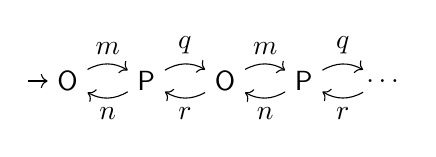
\begin{tikzpicture}[baseline=(O1.base)]
    \node (O1) at (0,0) {\kw{O}};
    \node (P1) at (1,0) {\kw{P}};
    \node (O2) at (2,0) {\kw{O}};
    \node (P2) at (3,0) {\kw{P}};
    \node (O3) at (4,0) {$\ldots$};
    \path [->] (-0.5,0) edge (O1);
    \path [->] (O1) edge[bend left] node[auto] {$m$} (P1);
    \path [->] (P1) edge[bend left] node[auto] {$n$} (O1);
    \path [->] (P1) edge[bend left] node[auto] {$q$} (O2);
    \path [->] (O2) edge[bend left] node[auto] {$r$} (P1);
    \path [->] (O2) edge[bend left] node[auto] {$m$} (P2);
    \path [->] (P2) edge[bend left] node[auto] {$n$} (O2);
    \path [->] (P2) edge[bend left] node[auto] {$q$} (O3);
    \path [->] (O3) edge[bend left] node[auto] {$r$} (P2);
  \end{tikzpicture}
  \quad
  \begin{array}{cc}
    m \in F & q \in E \\[1ex]
    n \in \kw{ar}(m) & r \in \kw{ar}(q)
  \end{array}
\]
The first move is always a question $m$ played by $\kw{O}$ in $F$.
The player $\kw{P}$ can conclude the current instance of $F$
with an answer $n$, or
initiate an instance of $E$
with a question $q$.
Then $\kw{O}$ can initiate a new instance of $F$
with another $m$, or
conclude any current instance of $E$
with an answer $r$.
This process goes on indefinitely.

Readers familiar with traditional game semantics
will recognize this description
as the \emph{well-bracketed} plays for the game ${!}E \multimap {!}F$
whose arena can be described as:
\[
  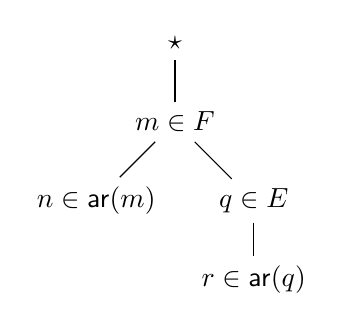
\begin{tikzpicture}
    \node (S) at (0,3) {$\star$};
    \node (BQ) at (0,2) {$m \in F$};
    \node (BA) at (-1,1) {$n \in \kw{ar}(m)$};
    \node (AQ) at (+1,1) {$q \in E$};
    \node (AA) at (+1,0) {$r \in \kw{ar}(q)$};
    \path (S) edge (BQ);
    \path (BQ) edge (BA);
    \path (BQ) edge (AQ);
    \path (AQ) edge (AA);
  \end{tikzpicture}
\]
However,
owing to the simplicity of $E$ and $F$,
our plays are much easier to describe
than in arena-based models.
Referring to the graph above,
we define the labelled transition system:
\[
  \begin{array}{rcccl}
    [x] & \xrightarrow{m \in F} & (m :: x)
        & \xrightarrow{n \in \kw{ar}(m)} & [x] \\
    (y) & \xrightarrow{q \in E} & [q :: y]
        & \xrightarrow{r \in \kw{ar}(q)} & (y)
  \end{array}
\]
The set of plays can then be defined as:
\[
  P_{E \rightarrow F} :=
    \{ \, s \mid \exists x \,.\,
       [\kw{nil}] \mathrel{{\xrightarrow{s}}{}^*} [x] \, \}
\]
Then writing $\sqsubseteq$ for the
obvious prefix ordering,
the morphisms from $E$ to $F$
can be constructed as:
\[
    \sigma \in \mathbf{FCD}(P_{E \rightarrow F}, {\sqsubseteq})
\]
We will write $\sigma : E \rightarrow F$.

\subsection{Composition}





%}}}

%}}}

\section{Refinement-based game semantics for C} %{{{

In this section we will give a quick overview of CompCertO
and explain how to use it in the context of our strategy model.

\subsection{Semantics of transition systems} %{{{

We now interpret the transition systems defined in \S\ref{sec:compcert}
in terms of the strategy model we have defined.
We consider a transition system $L : E \rightarrow F$
with the components $L = \langle S, {\rightarrow}, I, X, Y, F \rangle$.

In CompCert transition systems,
multiple transitions from a given state $s$
denotes demonic nondeterminism.
However,
the lack of any transition is interpreted as ``going wrong'',
in other words it denotes an undefined behavior.
To account for this idiom,
we define the notion of discontinuous choice among
a set $S \subseteq \mathcal{I}_E(A)$ of interactive computations:
\[
    \bigoplus S :=
    \begin{cases}
      \bot & \mbox{if } S = \varnothing \\
      \bigsqcap S & \mbox{otherwise}
    \end{cases}
\]
With this,
we can define the immediate behavior of a state $s \in S$ as
using the function $\delta : S \rightarrow \mathcal{I}_E(S)$
defined as:
\[
  \delta(s) :=
    \{ \kw{safe}(s) \} ;
    \left( \bigsqcap_{s \rightarrow s'} \eta(s') \right)
    \sqcap
    \left( \bigsqcap_{m \in X(s)} n \leftarrow \mathbf{I}(m) ;
            \bigoplus_{s' \in Y(s, n)} \eta(s') \right)
\]
The initial assertion ensures that unsafe states go wrong.
The subsequent demonic choice
collects transitions to other states,
either direct or after an interaction.
By iterating $\delta$, we can then compute the overall behavior of $L$:
\[
   \llbracket L \rrbracket (q) :=
     \bigoplus_{s \in I(q)}
     \left(
     \bigsqcup_{n \in \mathbb{N}}
     s' \leftarrow \delta^n(s) ; \bigsqcap_{r \in F(s')} \eta(r)
     \right)
\]

%}}}

\subsection{Simulation conventions} %{{{

Consider a simulation convention $\mathbb{R} : E_1 \Leftrightarrow E_2$
with the components $\mathbb{R} = \langle W, R^\kw{Q}, R^\kw{A} \rangle$.
We will define two adjoint strategies
which will translate questions and answers between
$E_1$ and $E_2$.
For purposes of intuition,
we can think of $E_1$ as the game $\mathcal{C}$,
$E_2$ as the game $\mathcal{A}$,
and $\mathbb{R}$ as the overall simulation convention of CompCert.

The strategy $\mathbb{R}^* : E_1 \rightarrow E_2$
is used to translate incoming calls
and is defined as follows:
\[
    \mathbb{R}^*(m_2) :=
       \bigsqcup_{m_1 \ifr{w \Vdash R^\kw{Q}} m_2}
       n_1 \leftarrow \mathbf{I}(m_1) ;
       \bigsqcap_{n_1 \ifr{w \Vdash R^\kw{A}} n_2}
       \eta(n_2)
\]
Note that the first choice ranges over the values of both
$w \in W$ and $m_1 \in M_{E_1}^\kw{Q}$,
whereas the second choice ranges only over the value of
$n_2 \in M_{E_2}^\kw{A}$.
If $m_2$ is an assembly call,
we first choose a corresponding C call $m_1$,
then pass the request along.
If there are no such calls,
the result is an undefined behavior.
When the answer $n_1$ is received,
we translate it back to an assembly return $n_2$.
The exact details of $n_2$ will be chosen by
the compiled program implementing our specification,
hence we use a demonic choice.

The strategy $\mathbb{R}_* : E_2 \rightarrow E_1$
is used to translate outgoing calls
and is defined as follows:
\[
    \mathbb{R}_*(m_1) :=
       \bigsqcap_{m_1 \ifr{w \Vdash R^\kw{Q}} m_2}
       n_2 \leftarrow \mathbf{I}(m_2) ;
       \bigsqcup_{n_1 \ifr{w \Vdash R^\kw{A}} n_2}
       \eta(n_1)
\]
Here,
the compiled system will determine
the details of the assembly call,
whereas its environment will determine
the exact assembly state returned.
Hence, the polarity of choices is reversed.

With these definitions,
given two simulation conventions
$\mathbb{R} : E_1 \Leftrightarrow E_2$ and
$\mathbb{S} : F_1 \Leftrightarrow F_2$,
we can give the concretization of a strategy
$\sigma \in \llbracket E_1 \rightarrow F_1 \rrbracket$
according to the simulation convention
$\mathbb{R} \rightarrow \mathbb{S}$
as the strategy
$\gamma_{\mathbb{R} \rightarrow \mathbb{S}}(\sigma) \in
  \llbracket E_2 \rightarrow F_2 \rrbracket$
defined by:
\[
    \gamma_{\mathbb{R} \rightarrow \mathbb{S}}(\sigma) :=
    \mathbb{R}^* \circ \sigma \circ \mathbb{S}_* \,.
\]

%}}}

\subsection{Soundness of simulations} %{{{

Putting these ingredients together,
backward simulations can be embedded as refinement:
\[
  \begin{prooftree}
    \hypo{L_1 \ge_{\mathbb{R} \rightarrow \mathbb{S}} L_2}
    \infer1{\gamma_{\mathbb{R} \rightarrow \mathbb{S}}
                (\llbracket L_1 \rrbracket) \sqsubseteq
                \llbracket L_2 \rrbracket}
  \end{prooftree}
\]
[Actually we could use forward sim directly,
interpreting all CompCert nondet as angelic,
which doesn't matter if we've shown they're determinate
and makes the embedding simpler.]

%}}}

\subsection{Compiler correctness} %{{{

Formulated in our setting as:
\[
    \gamma_{\mathbb{C} \twoheadrightarrow \mathbb{C}}
          (\llbracket \kw{Clight}(p) \rrbracket) \sqsubseteq
    \llbracket \kw{Asm}(p') \rrbracket
\]

%}}}

\subsection{Certified abstraction layers} %{{{

\paragraph{Defining layer specifications} %{{{

To define certified abstraction layers,
we can introduce a new construction is $A[S]$,
which roughly corresponds to the \emph{state monad transformer},
and adjoins a state $s \in S$ to both the questions and answers of $A$.
We can then define a state hiding operator:
\[
    \sigma : A[S] \rightarrow B[S] \vdash
    h(\sigma, s_0) : A \rightarrow B \,.
\]
The hiding operator keeps track of an internal state
initialized to $s_0$.
For every input (a question in $B$ or an answer in $A$),
$h$ adjoins the current state before passing it to $\sigma$.
For every output (an question in $A[S]$ or an answer in $B[S]$),
$h$ updates the current state with the one provided
before passing the remainder to the environment.

A $\mathcal{C}$ \emph{layer interface} is defined as
$L := \langle S, s_0, I, \sigma \rangle$,
where $S$ is the type of abstract states,
$s_0 \in S$ the initial abstract state,
$I \subseteq S$ an invariant and
$\sigma \in
 \gcat[\mathcal{C}\langle D \rangle, \mathcal{C}\langle D \rangle]$
gives the layer's specification.



Now we can use 
This allows us to define stateful strategies
using $S$ as 
using the convenience interaction monad:
$\sigma \in \gcat^i[A, B \langle S \rangle]$
to $\sigma^\dagger \in \gcat[A, B \langle S \rangle]$
to $h(\sigma^\dagger, s_0) \in \gcat[A, B]$.

%}}}

\paragraph{Abstraction relations} %{{{

From the usual match/relate relations
we can formulate a Galois connexion
similar to what happens with simulation conventions
(in fact we could probably define an actual simulation convention).
Then the goal is to show that for 

%}}}

%}}}

%}}}

\section{Related work} \label{sec:rw} %{{{

\begin{itemize}
\item nondeterminism in game semantics
\item ATL, alternating transition systems, alternating refinement
\item \ldots
\item order-theoretic \emph{concurrent games} worth looking at
  in this framework?
\end{itemize}

%}}}

\bibliographystyle{ACM-Reference-Format}
\bibliography{../references}

\end{document}
